\section{Cathode Signal Processing}
\label{sec:clct}

\subsection{CLCT Algorithm}
\label{subsec:clct_algo}

[We need a good picture illustrating CLCT processing process like in the case of ALCT one]

A muon passing through a CSC chamber will produce distinctive patterns of half-strip
hits in the six-layer endcap muon CSC chambers. By identifying these patterns, the CSC Local
Trigger provides high rejection power against backgrounds. The largest background source,
neutron-induced gamma ray conversions, are generally low in energy, and produce mostly single-
layer or short multi-layer hits. Other backgrounds, such as low-momentum muons or punch-
through particles often do not point well enough to the primary interaction region to be considered
high-momentum muon candidates.

\begin{figure}[tbh]
        \begin{center}
                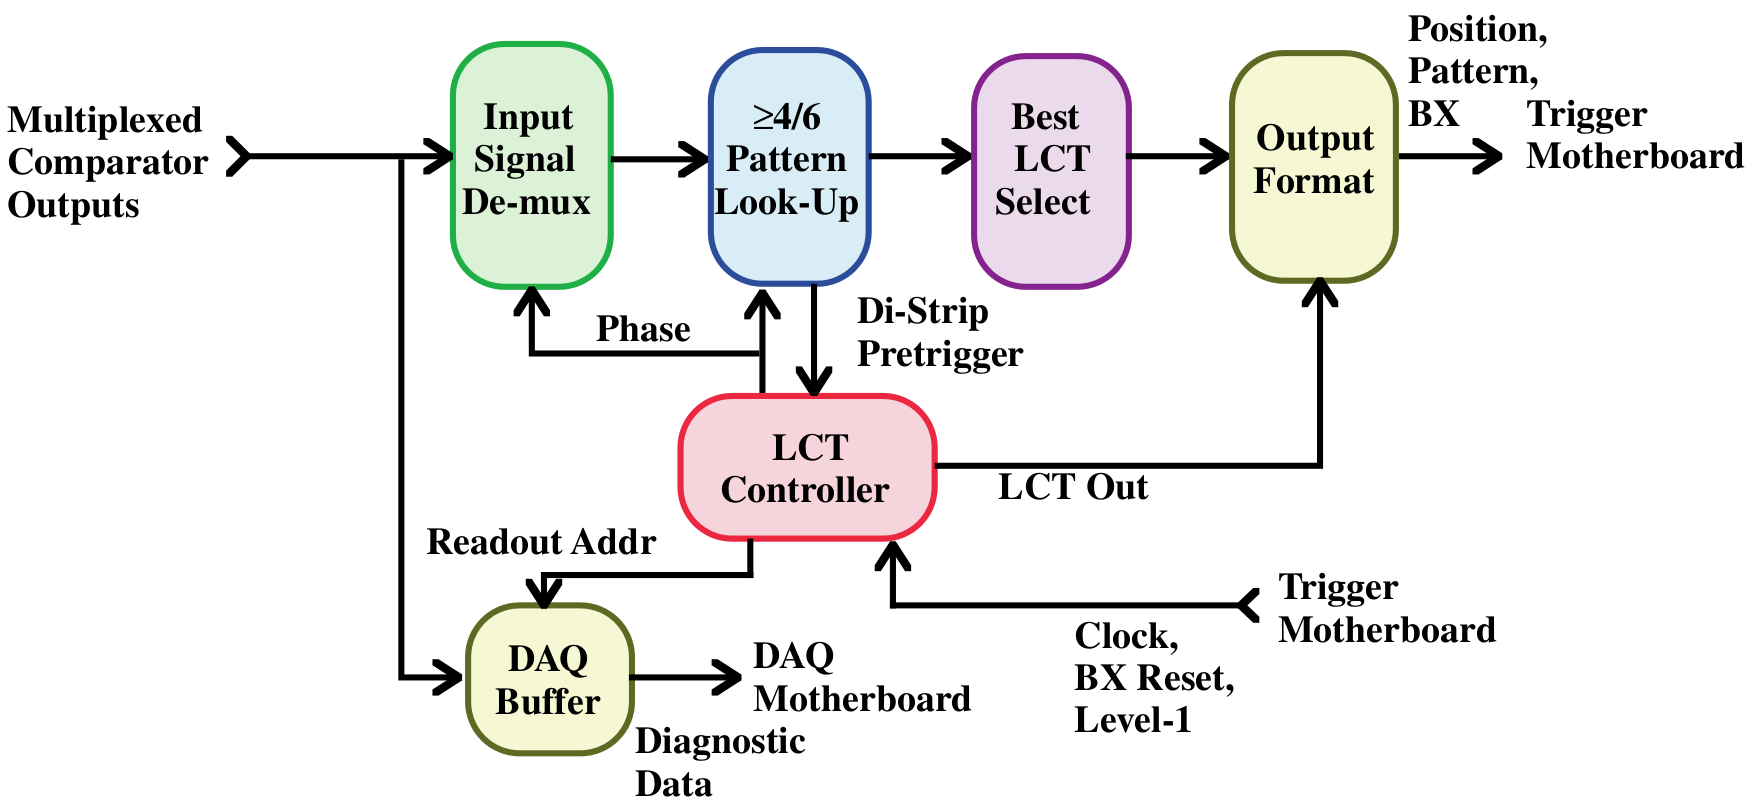
\includegraphics[width=0.73\linewidth]{figures/CLCT_block_diagram.png}
                \caption{CLCT block diagram}
                \label{fig:clct_block_diagram}
        \end{center}
\end{figure}

[Technical description from TMB manual below]

For each of 160 key half-strips consider the 42 neighboring half-strips (i.e. on key 5 use the following half-strips):

\begin{figure}[tbh]
        \begin{center}
                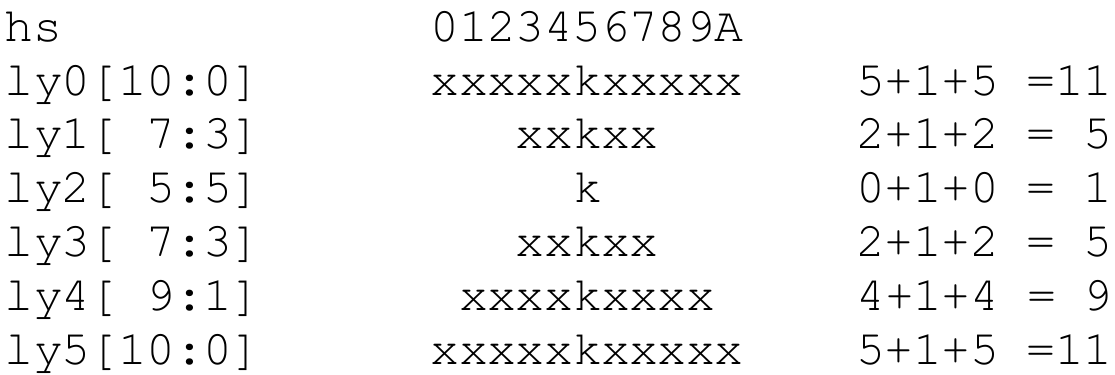
\includegraphics[width=0.48\linewidth]{figures/160_key_half_strips.png}
                \caption{160 key half-strips}
                \label{fig:160_key_half_strips}
        \end{center}
\end{figure}

For each of 160 key half-strips, count layers with hits matching the 9 pattern templates:

\begin{figure}[tbh]
        \begin{center}
                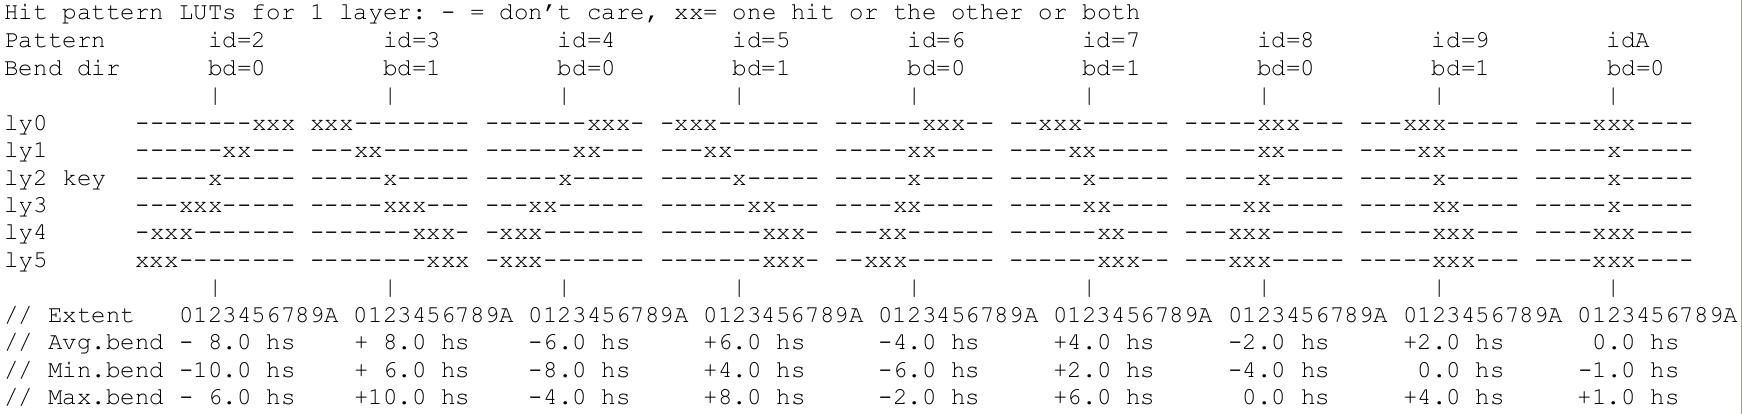
\includegraphics[width=0.98\linewidth]{figures/CLCT_patterns.png}
                \caption{CLCT patterns}
                \label{fig:clct_patterns}
        \end{center}
\end{figure}

Pattern ID=1 is a layer-OR trigger, Pattern ID=0 is no-pattern-found. Result for each of 160 keys is a list of 9 pattern-ID numbers (pid) [2 to A] and corresponding
number of layers [0 to 6] with matching hits (nhits). Find the best 1-of-9 pattern ID numbers for each key by comparing nhits. Ignore bend direction: left and right bends have equal priority (bit 0 of pid implies bend direction).
If two pattern IDs have the same nhits, take the higher pattern ID. A key with no matching hits, would always return pid=A and nhits=0.
Pre-trigger if any 1-of-160 keys have nhits $\geq$ hit\_thresh\_pretrig and pid $\geq$ pid\_thresh\_pretrig.

Construct 7-bit pattern quality pat[7:0] for sorting where pat[7:5]=nhits[2:0], pat[4:0]=pid[3:0]. Ignore the bend direction bit (pid[0]), left and right bends have equal priority. 
Store pat[7:0] for 160 keys for use later to find 2nd CLCT.
Find the best key out 1-of-160 keys by sorting on the 6-bit number pat[7:1]. Store 1st CLCT info: key, pattern ID, and number of hits.
For empty events, key=0, pid=A and nhits=0. If clct\_blanking=1, then key=pid=hits=0.

Mark keys near 1st CLCT as busy from 1st key-nspan to 1st key+pspan.
If clct\_sep\_src=1, pspan and nspan are set equal to clct\_sep\_vme, typically 10 half-strips.
If clct\_sep\_src=0, pspan and nspan are read from RAM and depend on the pattern ID number, this allows two less bending tracks to be closer than more bending tracks.

Find the best key out of 1-of-160 keys by sorting on the 6-bit number pat[7:1]: skip busy keys, if two keys have the same pat[7:1] take the lower key.
Store the same information for the 2nd CLCT as for the 1st one.

Wait for CSC drifting (drift delay of 2BXs) and perform matching to ALCTs.


\subsection{Separation of the CLCTs in ME1/1a and ME1/1b}

In the old TMB f/w, the 16 ganged strip channels from ME1/1a are appended to the 64 ME1/1b strip channels and the reconstruction of CLCTs is performed as if it's a single regular chamber with 80 channels (is there any treatment of the boundary, so that ME1/1a strips are not combined with ME1/1b strips?). The two rather separate and distinctive areas combined and treated like one uniform unit with the maximum of two CLCT stubs on the output.

With unganged ME1/1a and higher pile-up such a simple approach becomes increasingly unnatural and ineffective. The ME1/1a would have x3 more channels now, so it would deserve to be treated like a separate chamber even more. And chances to get multiple stubs are increasing with higher luminosity, especially so in ME1/1a. With multiple stubs, the stubs in ME1/1a would start directly competing with those in ME1/1b.

With a larger size FPGA, it would be beneficial to treat ME1/1a and ME1/1b as two separate chambers for the purpose of CLCT reconstruction, with each area having their own limit on the maximum of 2 CLCTs. Thus, the whole ME1/1 would be able to have maximum 4 CLCTs available for matching with ALCTs. It's important to keep more 2D stubs available so that at the stage of matching we can reduce the number of stubs following some better tuned criteria.

Finally, in the case if we would allow to read out the 2D CLCT stubs without an ALCT match, and we cannot read out more then 2 of them per BX per ME1/1, we can device a selection criteria when comparing stubs from ME1/1a and ME1/1b as follows: e.g., if quality of an ME1/1b stub is the same or less by one then that of an ME1/1a stub, prefer the ME1/1b one. 

\subsection{Localization of the TMB Dead Time}

 The main source of the old TMB inefficiency in high pile-up is the dead time which happens for the whole ME1/1 chamber after there was a triggering CLCT. The TMB's state-machine freezes whole TMB for several BXs after a CLCT trigger while number of coincidence layers stays over the trigger threshold. If anywhere in a chamber there was an CLCT from PU a few BX earlier before a signal muon, it would be impossible to trigger on the signal.

While it's clear that with the comparator information which we recieve in TMB, it's not really possible to distinguish close in time signals in the same strip, there seem to be no apparent reason, other then the complexity of the algorithm, for this dead time to be present in strips that had no trigger.

Thus, the algorithm approach to deal with this issue for the upgrade could be as follows:
\begin{itemize}
    \item when a CLCT trigger happens, mark as busy only those strips within either a fixed dead time zone around CLCT (8 half-strips, see "useDeadTimeZoning" parameter in Sec.~\ref{sec:CLCT_conf}) or within the dead time zone, the width of which depends on the CLCT pattern (from 11 half-strips for the most bent patterns to 3 half-strips for the straightest one, see "useDynamicStateMachineZone" parameter in Sec.~\ref{sec:CLCT_conf}), and also mark the signal half-strip that specifies the triggered CLCT
    \item during the following bunch-crossings, check if the number of coincidence layers drops under the trigger threshold for the signal half-strip
    \begin{itemize}
	\item if it does, remove the "busy" mark from the corresponding strips 
    \end{itemize}
    \item if strips are marked as busy in a BX, they are excluded from pattern recognition 
\end{itemize}

\subsection{Restriction on the CLCT Pattern Bend}

The current set of CLCT patterns (see details in Sec.~\cite{subsec:clct_algo}) is largely geared towards low pt tracks. For tracks with pt>10, only the straighest and the next one bent patterns are significant. The restriction on allowed pattern bending would significantly help with many issues including multiplicity \& rate, ghosting, dead-time and corresponding loss of the efficiency (see "clctPidThreshPretrig" parameter in Sec.~\ref{sec:CLCT_conf}). Positive effect of it would increase with increasing luminosity. However, it would also somewhat reduce the efficiency because of not so good pt-threshold resolution from fairly narrow (11cm) CSC chambers, especially for medium to lower pt muons.

Plots on Fig.~\ref{fig:efficiency_vs_pt} show the efficiency vs $p_T$ for a simulated muon track to have a matching reconstructed CLCT stub for different sets of patterns (which defines maximum thresholds for the bend). Note, that adding GEMs could be helpful for improving the the efficiency of the bend restriction.

\begin{figure}[tbh]
        \begin{center}
                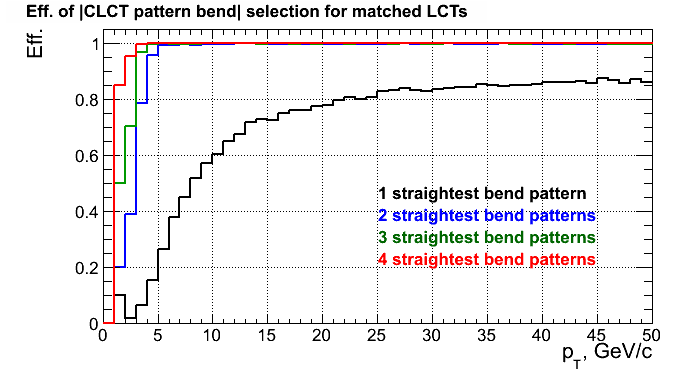
\includegraphics[width=0.48\linewidth]{figures/efficiency_vs_pt.png}
                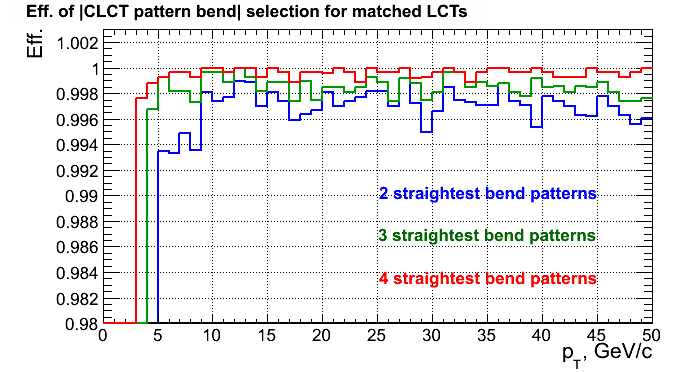
\includegraphics[width=0.48\linewidth]{figures/efficiency_vs_pt_scale.png}
                \caption{Efficiency vs $p_T$. No pile up is included in the simulated sample.}
                \label{fig:efficiency_vs_pt}
        \end{center}
\end{figure}

\subsection{Improvement of the CLCT Timing}

Currently, the BX time of a CLCT stub is defined as the BX of its pretrigger. Or, in other words, it's first BX when at least three layers fit one of the CLCT patterns. Note that an attempt to latch a trigger pattern is performed after the number of BX after the pretrigger defined by the clctDriftDelay parameter (=2BX). And also note that a CLCT pattern during the pretrigger could be different then the one that happen to match during the trigger.

With higher luminosity there are increasingly larger chances for some strips in some of the layers to be hit by earlier background hit. And that has chances to affect the time when a pretrigger might be detected. A more robust solution would be to define stub's time using the times of its strips, where stub's strips are defined as strips that were matched within a CLCT pattern during the trigger. As for a specific procedure, a median time over those strips' times or some sort of a truncated average could be used (see "clctUseCorrectedBx" parameter in Sec.~\ref{sec:CLCT_conf}, analogously for "alctUseCorrectedBx" parameter in Sec.~\ref{sec:ALCT_conf}).

\newpage
\subsection{Software Emulation of CLCT Processing}

CLCT processing includes the following four steps:

\begin{itemize}
    \item Pulse extension;
    \item Pretrigger;
    \item Trigger;
    \item CLCT construction and CLCT dead time.
\end{itemize}

In contrast to ALCT processing, where all steps are independent and performed one after another for all 16 BXs, during CLCT processing last three steps repeated in one global loop over BXs.

\subsubsection{Pulse Extension}

Sofware emulation provides information about all half-strip signals in DAQ readout window (16 BXs). A search for these signals is performed in a loop over all half-strips, all layers, and all 16 BXs; found signals are stretched over 6 BXs (see Fig.~\ref{fig:clct_pulse_extension}).

\begin{figure}[tbh]
        \begin{center}
                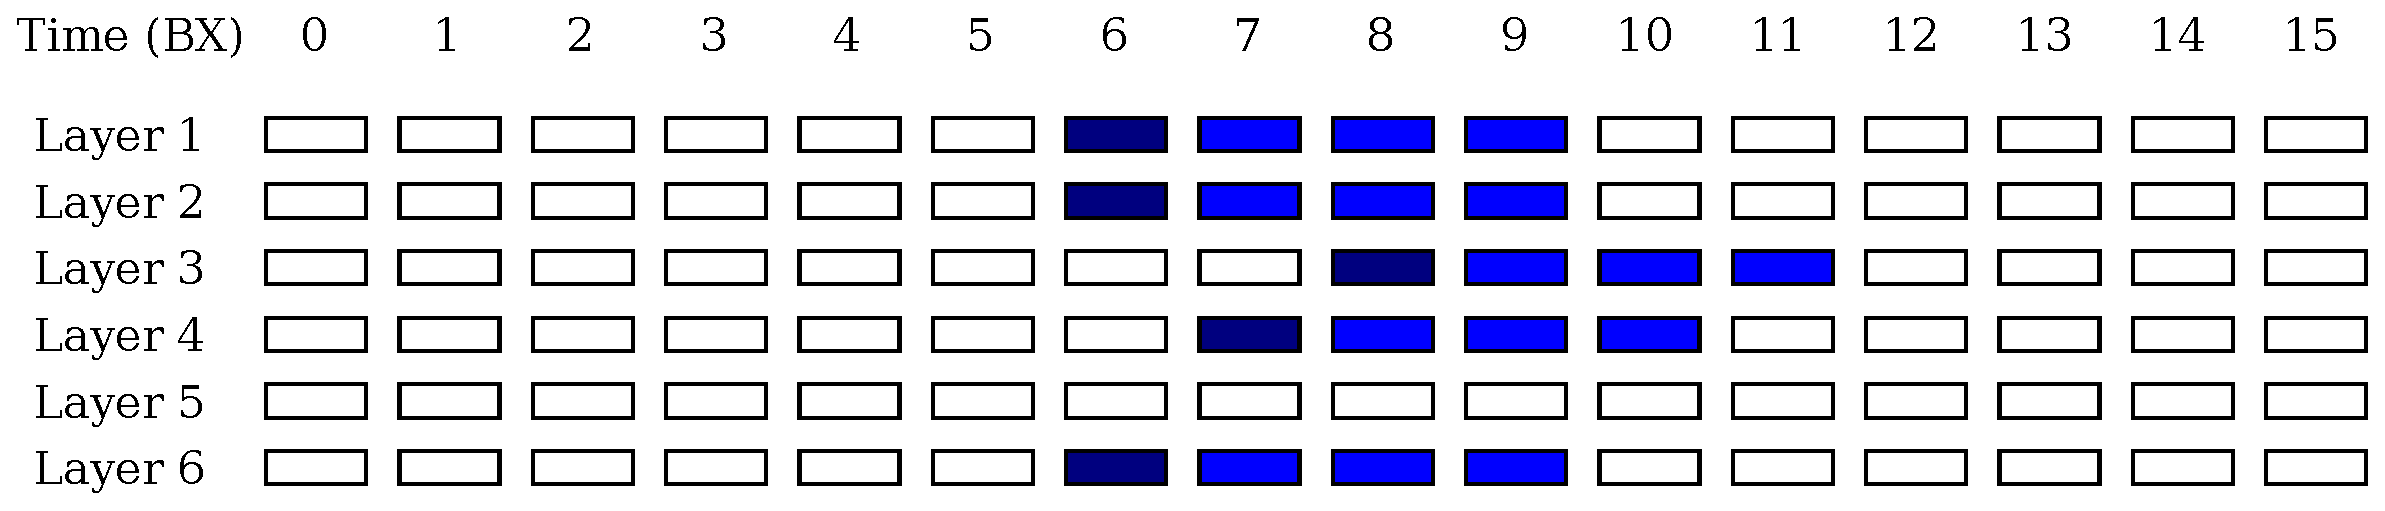
\includegraphics[width=0.9\linewidth]{figures/stretched_hits_clct.pdf}
                \caption{Illustration of ALCT pulse extension for one specific half-strip.}
                \label{fig:clct_pulse_extension}
        \end{center}
\end{figure}

\subsubsection{Pretrigger}

After all available half-strip signals are stretched, start a global loop over all BXs from BX = 0 and search for CLCT pretriggers in all half-strips. For any given BX and half-strip, count the number of layers with hits within the patterns shown on Fig.~\ref{fig:clct_pretrigger}, and if this number is greater than or equal to three, then we say that a pretrigger occured in this BX and this half-strip. This pretrigger is only accepted if its pattern id $\geq$ 2. If there were no CLCTs found in some BX = B, proceed to BX = B+1 and continue searching for pretriggers. If there are some CLCTs found in the current BX, proceed to next step.

\begin{figure}[tbh]
        \begin{center}
                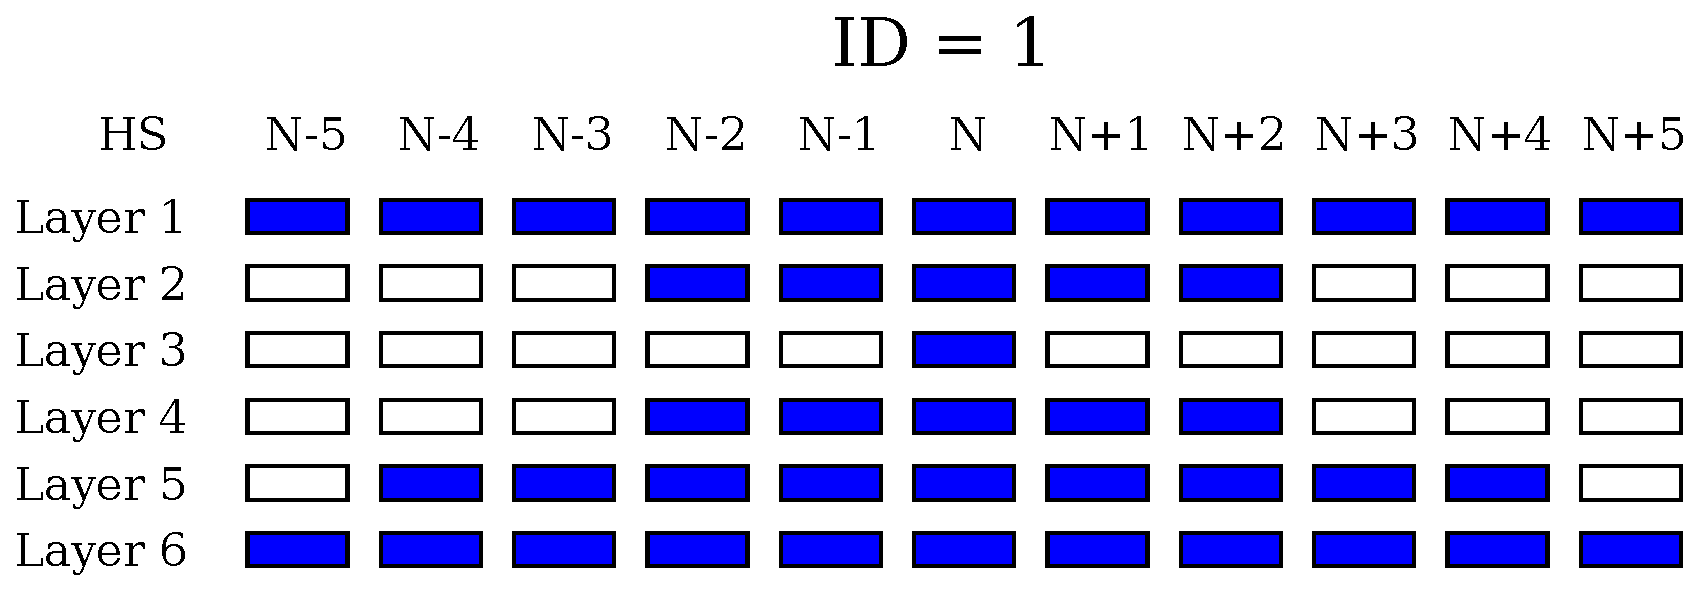
\includegraphics[width=0.48\linewidth]{figures/clct_pattern_01.pdf}
                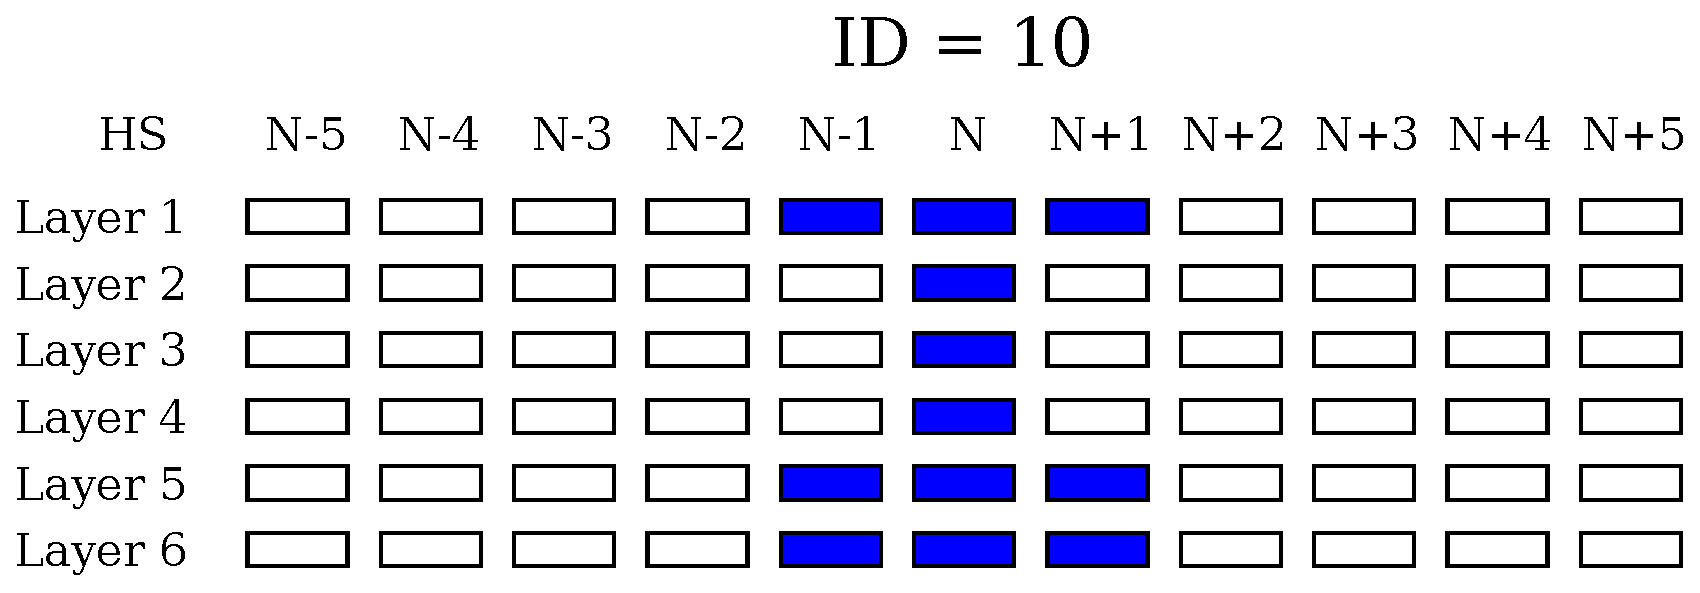
\includegraphics[width=0.48\linewidth]{figures/clct_pattern_10.pdf}\\
                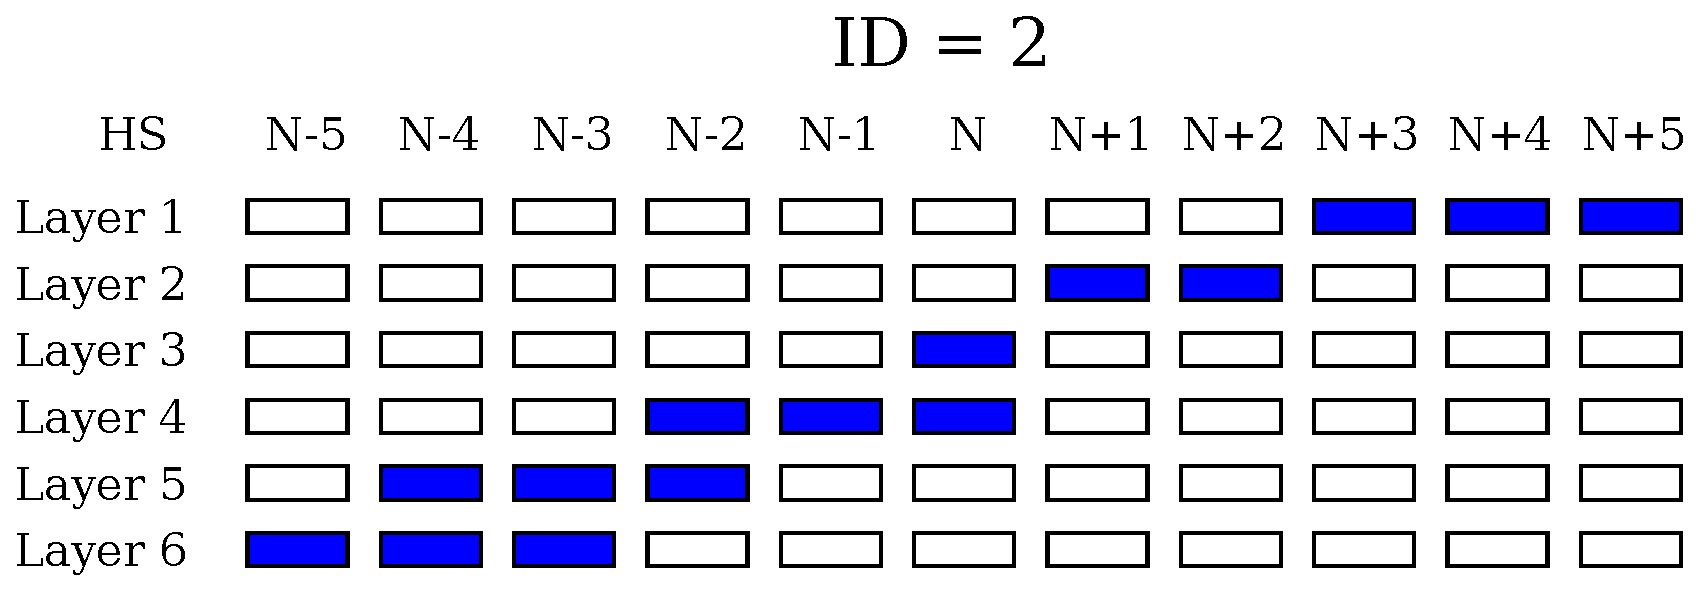
\includegraphics[width=0.48\linewidth]{figures/clct_pattern_02.pdf}
                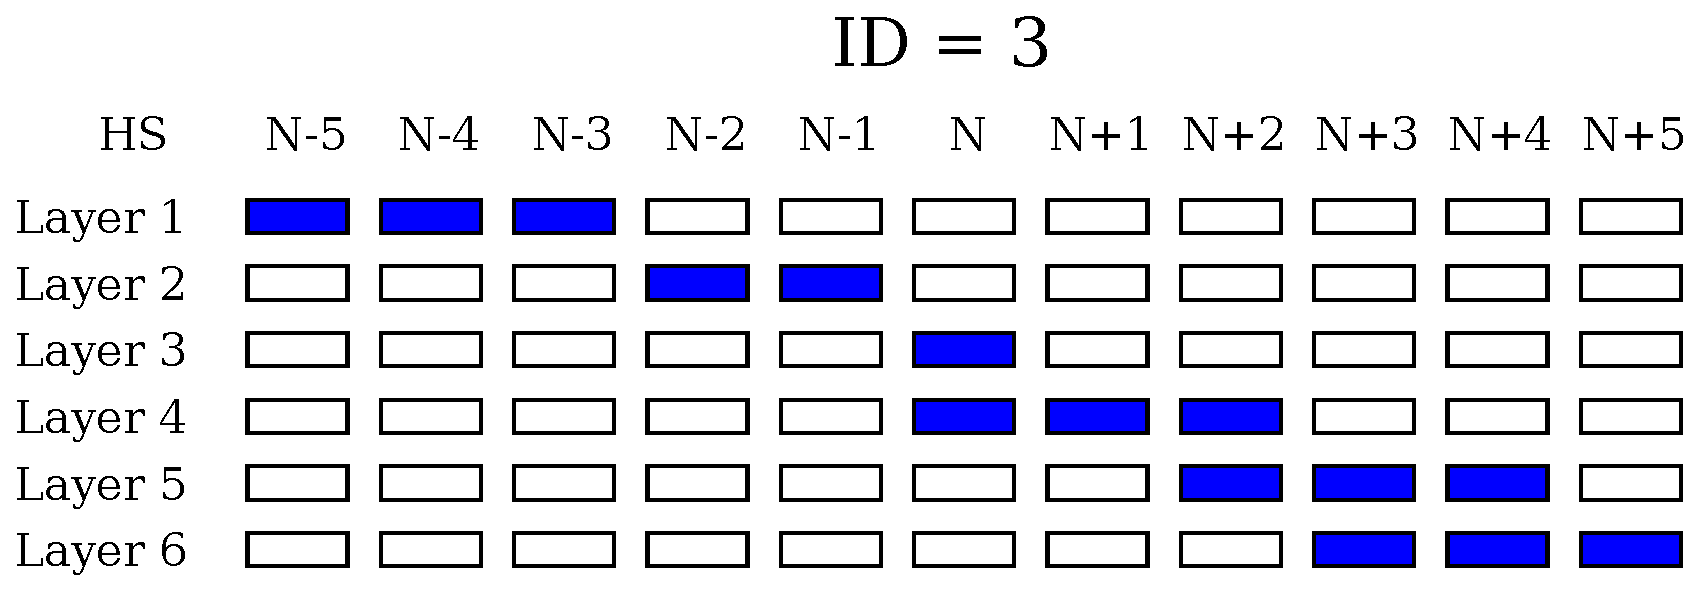
\includegraphics[width=0.48\linewidth]{figures/clct_pattern_03.pdf}\\
                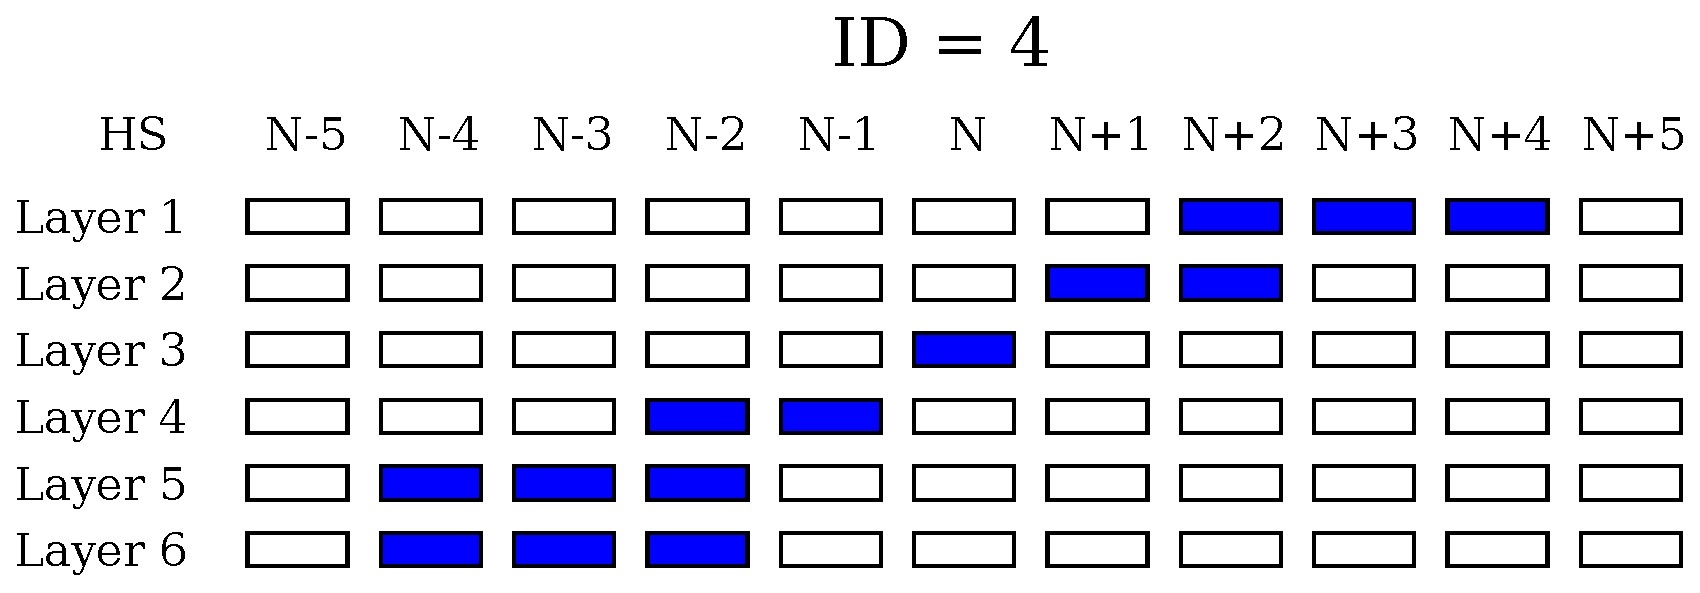
\includegraphics[width=0.48\linewidth]{figures/clct_pattern_04.pdf}
                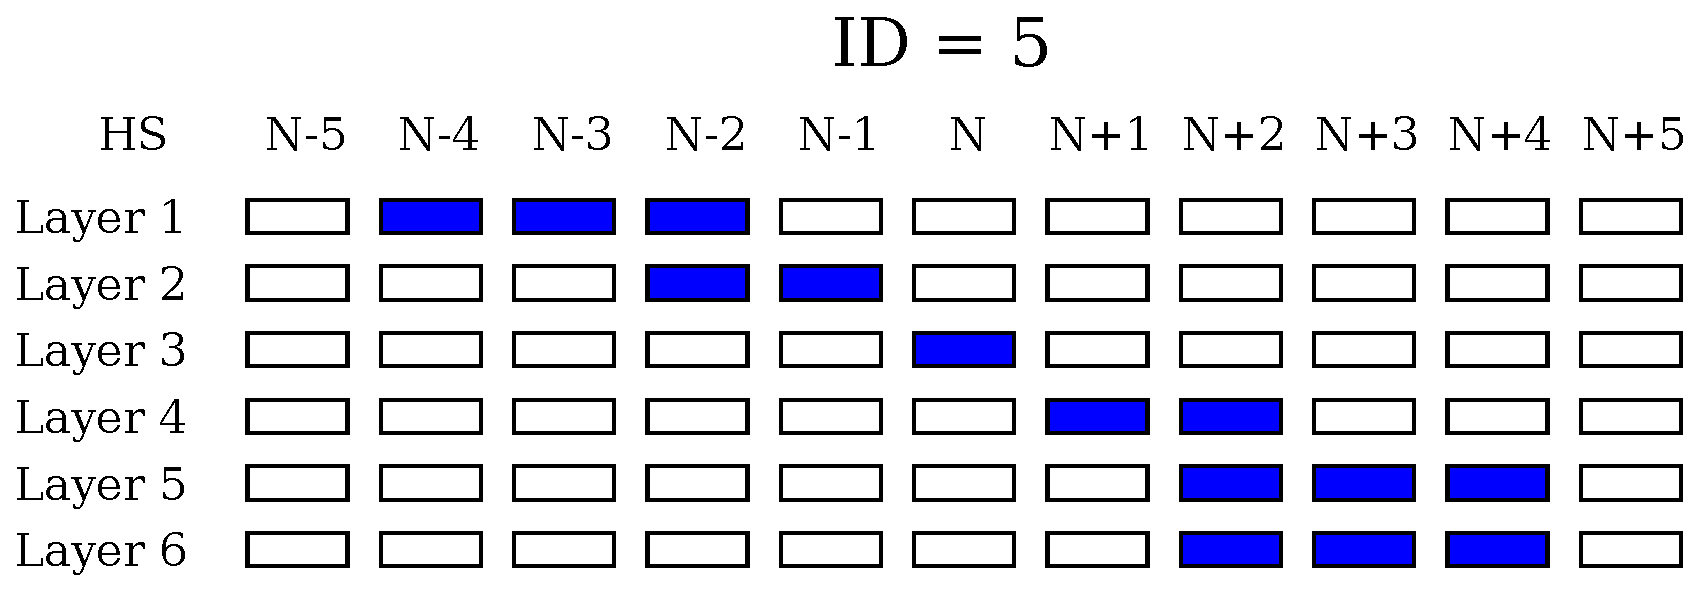
\includegraphics[width=0.48\linewidth]{figures/clct_pattern_05.pdf}\\
                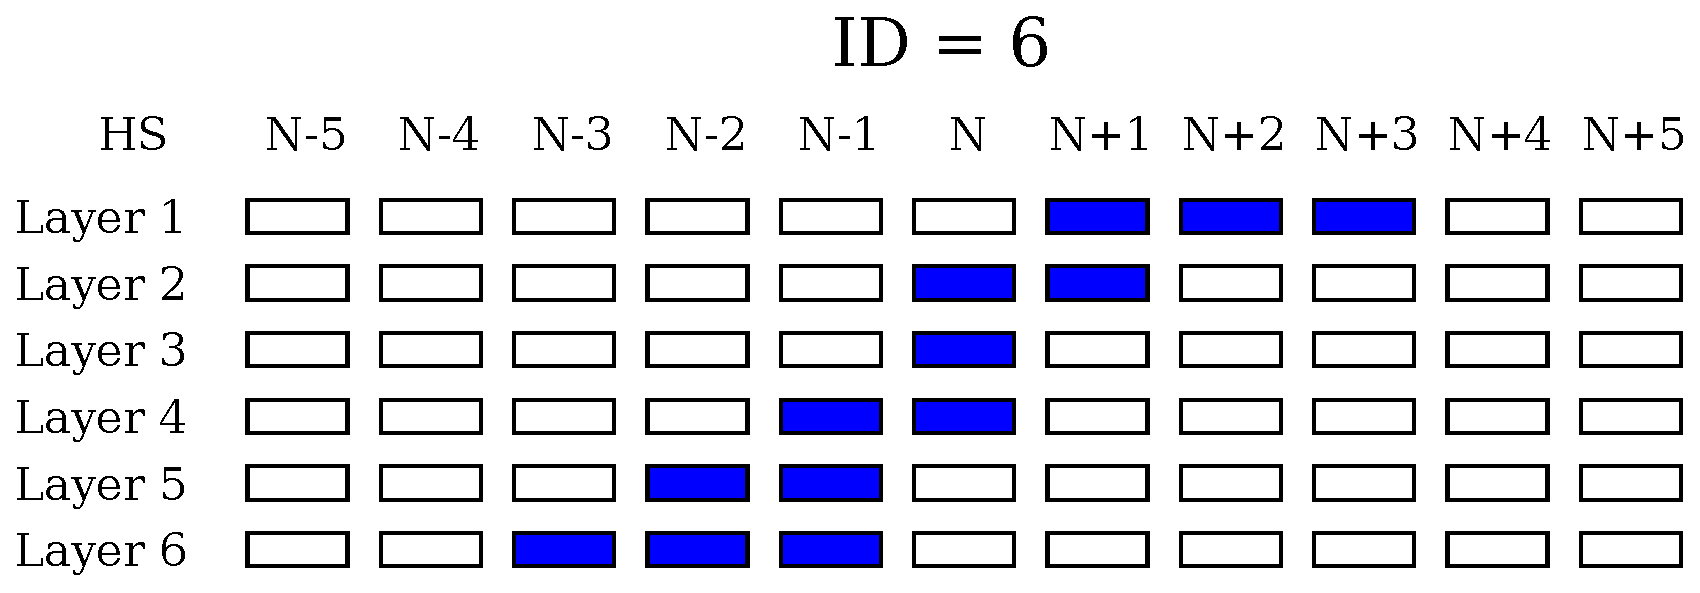
\includegraphics[width=0.48\linewidth]{figures/clct_pattern_06.pdf}
                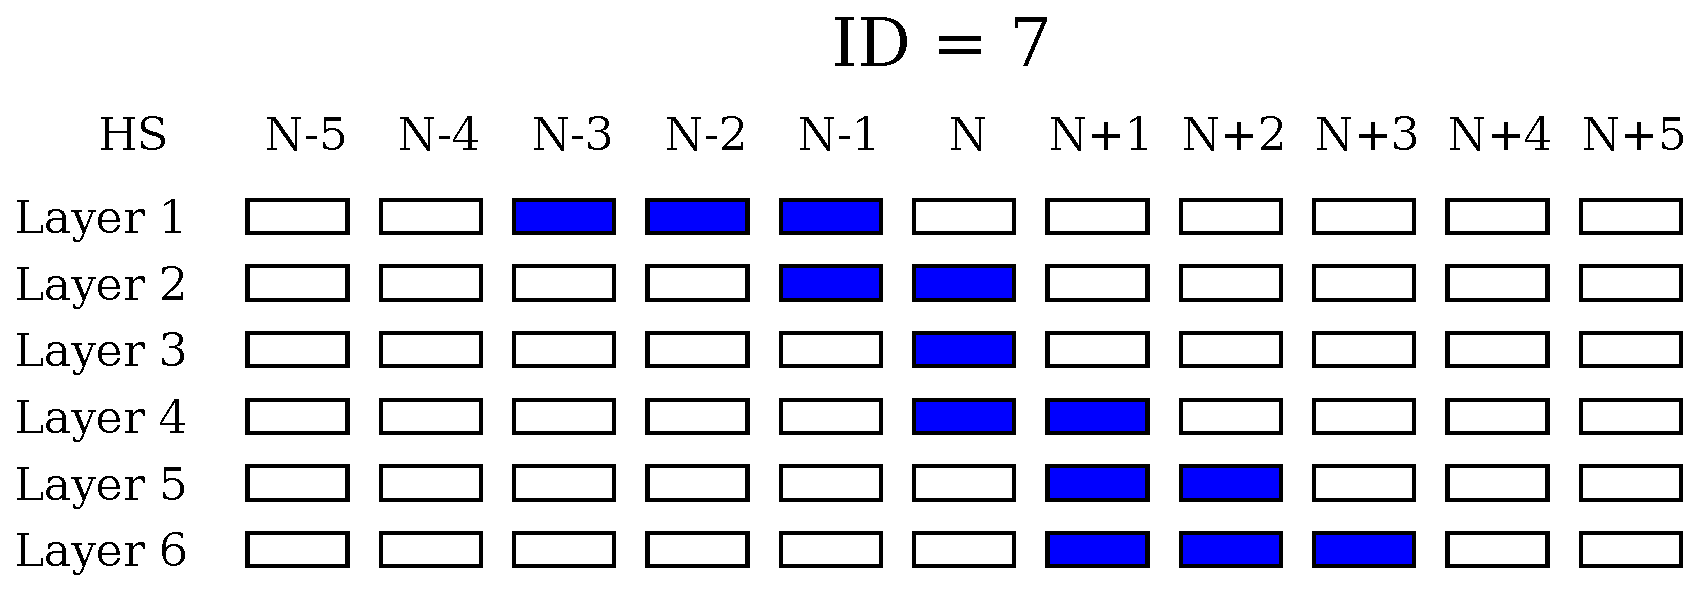
\includegraphics[width=0.48\linewidth]{figures/clct_pattern_07.pdf}\\
                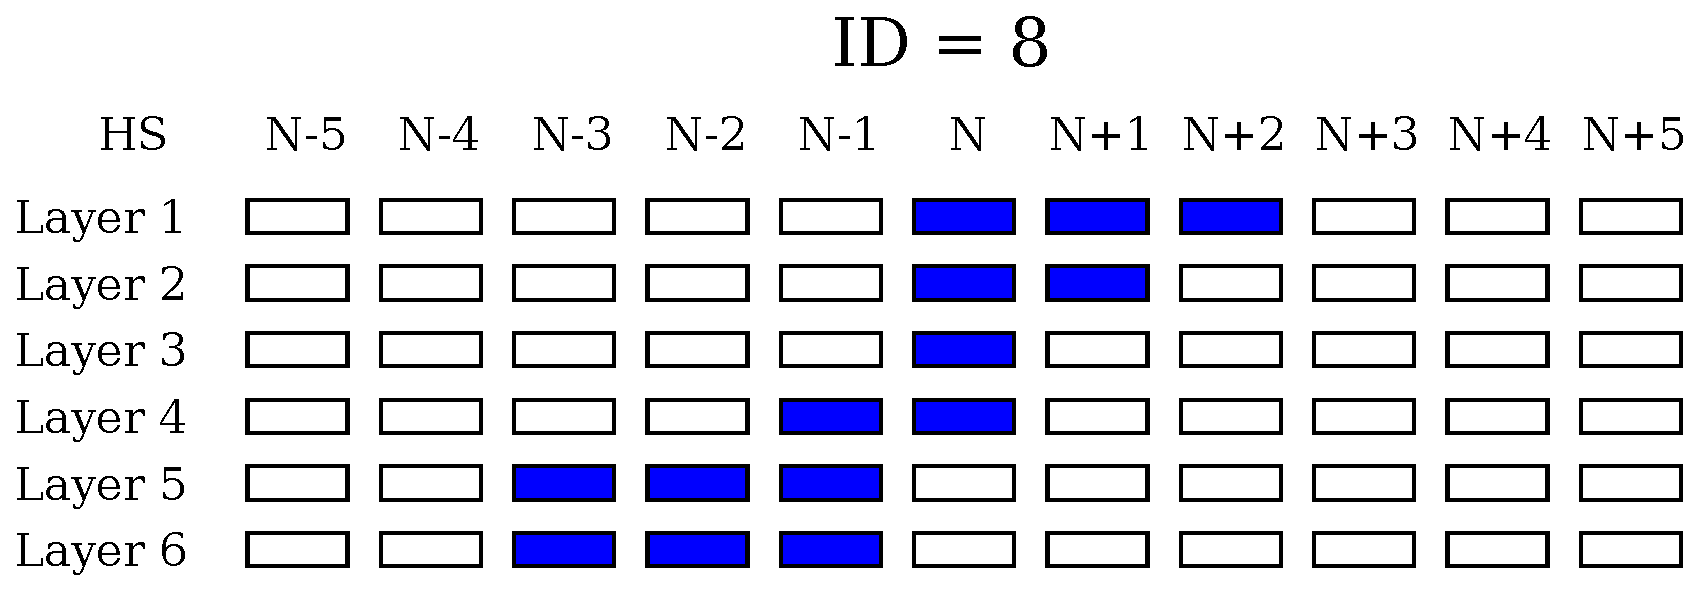
\includegraphics[width=0.48\linewidth]{figures/clct_pattern_08.pdf}
                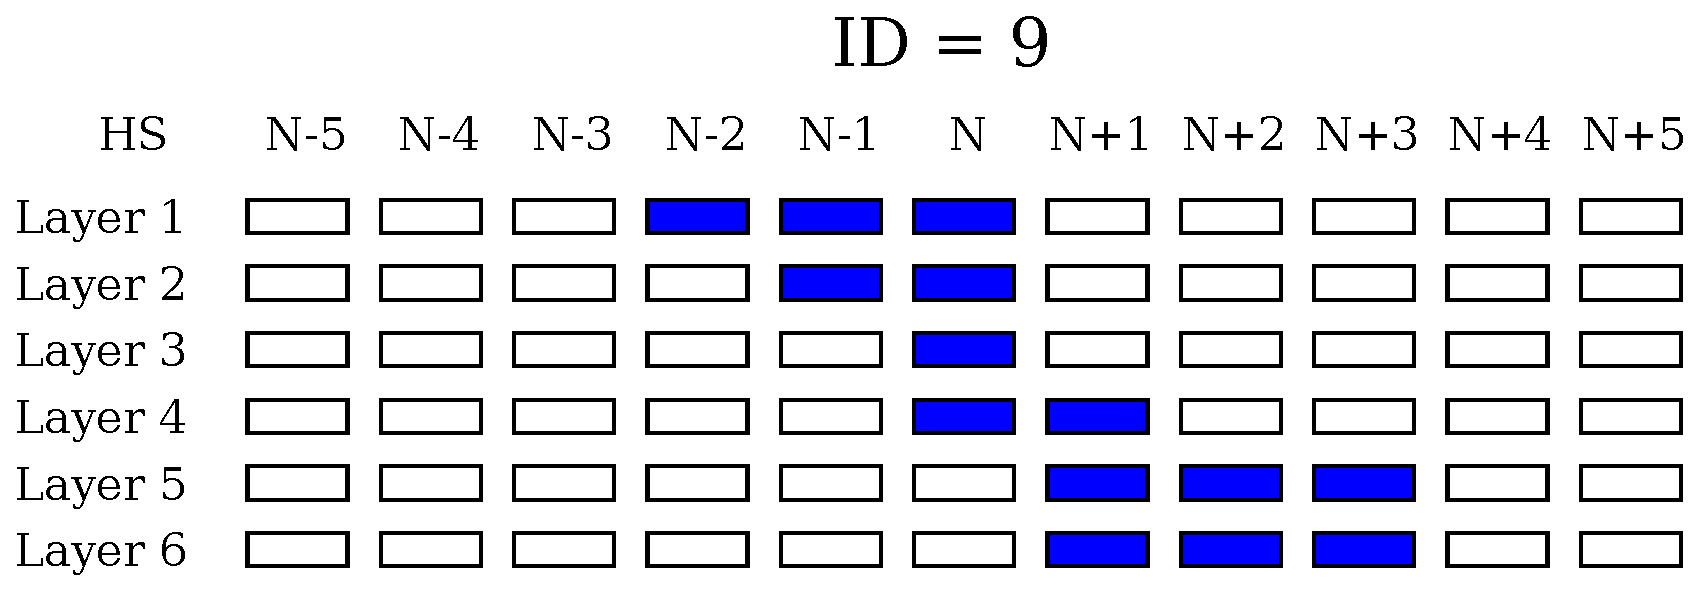
\includegraphics[width=0.48\linewidth]{figures/clct_pattern_09.pdf}
                \caption{CLCT patterns for pretriggering and triggering.}
                \label{fig:clct_pretrigger}
        \end{center}
\end{figure}

\subsubsection{Trigger}

As soon as a BX = B with CLCT pretrigger(s) is found, search for triggers in BX = B+2. For each half-strip, count the number of layers with hits within the same patterns used for pretriggering, and if this number is greater than or equal to four, we say that a trigger occured in this half-strip and BX, and remember:
\begin{itemize}
    \item pattern id with the highest number of hit layers (if there are two pattern ids with the same number of hit layers, choose smaller pattern id);
    \item number of hit layers in this pattern id.
\end{itemize}

Proceed to next step.

\subsubsection{CLCT Construction and CLCT Dead Time}

In a BX with CLCT triggers, find up to two best triggers to be used in CLCT construction.

Find the best trigger:
\begin{itemize}
    \item Find trigger with the highest number of hit layers;
    \item If there are two triggers with the same number of hit layers: choose the one with higher pattern id;
    \item If there are two triggers with the same number of hit layers and the same pattern id: choose the one with smaller half-strip.
\end{itemize}

Mark zone of 20 half-strips around the best trigger as used and find the second best trigger among not used half-strips.

Construct up to two best CLCTs from found best triggers: encode quality, pattern, bending direction, half-strip, cfeb, BX (defined by pretrigger BX).

After CLCT construction, keep CLCT "dead": continue the loop over all BXs until there is a BX with no triggers. When such a BX is found go back to pretriggering step.


\newpage
\subsection{Sofware Emulation of CLCT Level Improvements}

\subsubsection{Localizing Dead Zone}

\textcolor{red}{Current implementation of dead time}:
\begin{itemize}
    \item After constructing up to two CLCTs, \textcolor{red}{continue the loop over all BXs until there is a BX with no triggers}
    \\...
    \item In the BX with trigger, construct up to two CLCTs from two best triggers \textcolor{red}{in all half-strips}
    
\end{itemize}
\textcolor{blue}{New implementation of dead time}:
\begin{itemize}
    \item After constructing up to two CLCTs, \textcolor{blue}{mark 16 half-strips around half-strips of these CLCTs as busy while number of hit layers in half-strips of these CLCTs $\geq$ 4}
    \item \textcolor{blue}{After trigger in BX = B, keep searching for pretrigger in strating from BX = B+1}
    \\...
    \item In the BX with trigger, construct up to two CLCTs from two best triggers \textcolor{blue}{in half-strips}
    \begin{itemize}
        \item \textcolor{blue}{within 5 half-strips from pretrigger half-strips}
        \item \textcolor{blue}{which are not marked as busy from previous trigger}
    \end{itemize}
\end{itemize}

The following modifications in configuration are related to this improvement:
\begin{itemize}
    \item useDeadTimeZoning: False to True
\end{itemize}

\subsubsection{Dynamic Dead Zone Width}

\textcolor{red}{Fixed dead time zone}:
\begin{itemize}
    \item After constructing up to two CLCTs, mark \textcolor{red}{16} half-strips around half-strips of these CLCTs as busy while number of hit layers in half-strips of these CLCTs $\geq$ 4
\end{itemize}
\textcolor{blue}{Dynamic dead time zone}:
\begin{itemize}
    \item After constructing up to two CLCTs, mark \textcolor{blue}{K(pid)} half-strips around half-strips of these CLCTs as busy while number of hit layers in half-strips of these CLCTs $\geq$ 4
\end{itemize}
\vskip3mm
K(pid) --- function of pattern id:
\begin{itemize}
    \item K(1,2,3) = 22 half-strips
    \item K(4,5) = 18 half-strips
    \item K(6,7) = 14 half-strips
    \item K(8,9) = 10 half-strips
    \item K(10) = 6 halt-strips
\end{itemize}

The following modifications in configuration are related to this improvement:
\begin{itemize}
    \item useDynamicStateMachineZone: False to True
\end{itemize}

\newpage

\subsubsection{Minimal Pattern ID for Pretriggering}

\textcolor{red}{Current CLCT pretrigger}:
\begin{itemize}
    \item Loop over all BXs (starting from BX = 0) and all half-strips:
    \begin{itemize}
        \item Count number of layers with hits in the following patterns
        \item If this number $\geq$ 3: pretrigger occurs
        \item Accept this pretrigger if its pattern id $\geq$ \textcolor{red}{2}
    \end{itemize}
\end{itemize}
\textcolor{blue}{New CLCT pretrigger}:
\begin{itemize}
    \item Loop over all BXs (starting from BX = 0) and all half-strips:
    \begin{itemize}
        \item Count number of layers with hits in the following patterns
        \item If this number $\geq$ 3: pretrigger occurs
        \item Accept this pretrigger if its pattern id $\geq$ \textcolor{blue}{4}
    \end{itemize}
\end{itemize}

The following modifications in configuration are related to this improvement:
\begin{itemize}
    \item clctPidThreshPretrig: 2 to 4
\end{itemize}

\subsubsection{Minimal Separation Between Two Best CLCTs}

\textcolor{red}{Current construction of up to two CLCTs}:
\begin{itemize}
    \item Search for the best trigger in this BX
    \item Mark \textcolor{red}{20} half-strips around the best trigger as busy
    \item Find the second best trigger among non-busy half-strips
\end{itemize}
\textcolor{blue}{New construction of up to two CLCTs}:
\begin{itemize}
    \item Search for the best trigger in this BX
    \item Mark \textcolor{blue}{10} half-strips around the best trigger as busy
    \item Find the second best trigger among non-busy half-strips
\end{itemize}

The following modifications in configuration are related to this improvement:
\begin{itemize}
    \item clctMinSeparation: 10 to 5 cathode strips
\end{itemize}


\subsection{Results of Improvements of the CLCT Processing}

Improvements on the level of CLCT processor are related to the following configuration parameters (see Sec.~\ref{sec:CLCT_conf}):
\begin{itemize}
	\item useDeadTimeZoning: False to True;
	\item useDynamicStateMachineZone: False to True;
	\item clctPidThreshPretrig: 2 to 4;
	\item clctMinSeparation: 10 to 5 cathode strips.
\end{itemize}

Fig.~\ref{fig:CLCT_improvements_CLCT_recoEff} shows reconstruction efficiency of a good CLCT in ME1/1 station versus pseudorapidity of the simulated muon for different L1 configurations. The good CLCT is defined as CLCT:
\begin{itemize}
        \item read out in the window of 3BX around the central BX (BX6);
        \item reconstructed within 2 cathode strips from the key strip.
	\item has hits at least on four layers
\end{itemize}

The major improvement in CLCT reconstruction efficiency comes from localization of the deadtime zone.

\begin{figure}[p]
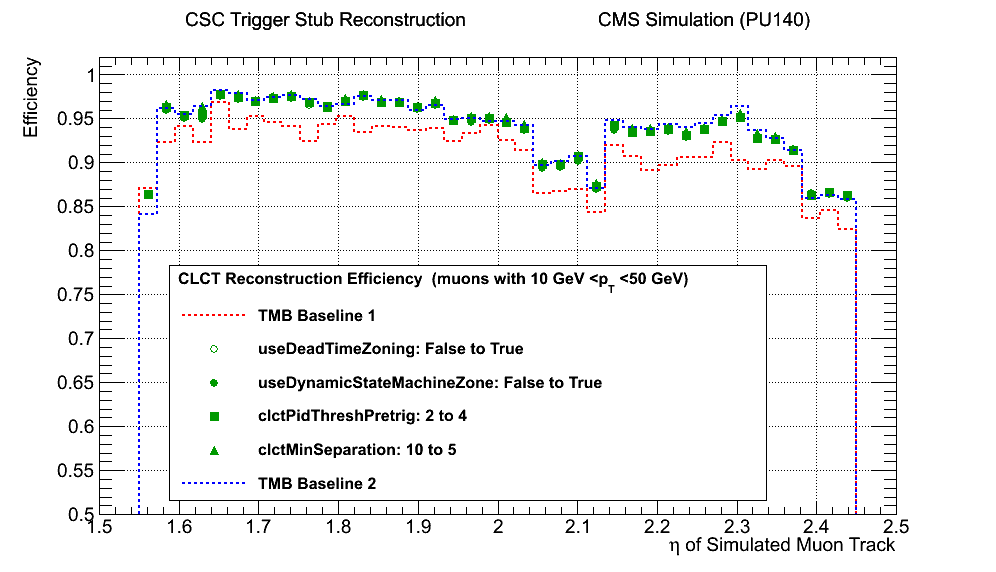
\includegraphics[width=0.98\textwidth]{figures/CLCT_improvements_CLCT_recoEff.png}
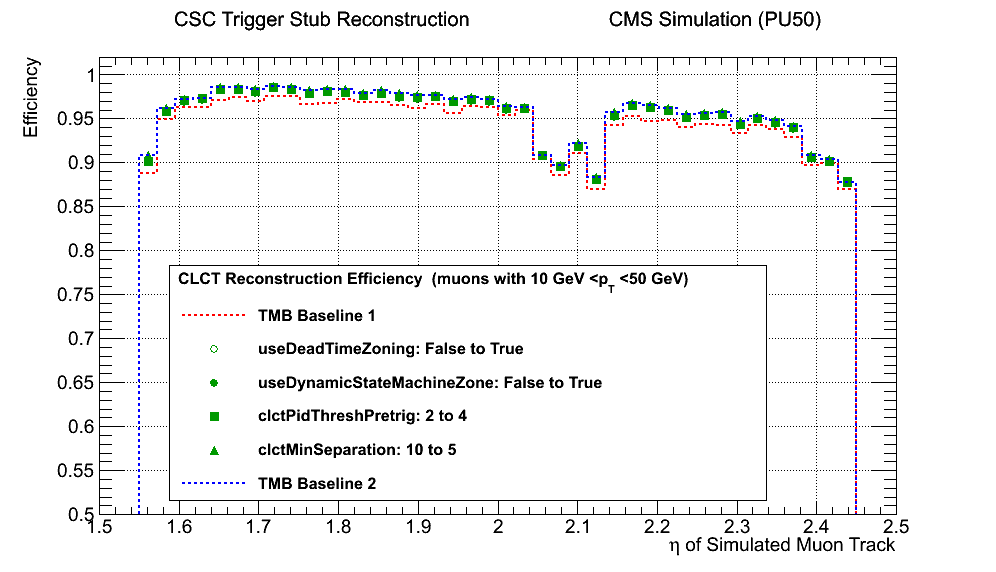
\includegraphics[width=0.98\textwidth]{figures/CLCT_improvements_CLCT_recoEff_PU50.png}
\caption{CLCT reconstruction efficiency in ME1/1 station for PU140 (top) and PU50 (bottom). Muons with transverse momentum $10$~GeV$<p_T<50$~ GeV are used in the analysis.}
\label{fig:CLCT_improvements_CLCT_recoEff}
\end{figure}